\documentclass[12pt,a4paper]{article}

\usepackage[dutch]{babel}
\usepackage{listings}

% Voor algoritmes
\usepackage{algorithm2e}

% Voor todo's
\usepackage{todonotes}

% font
\usepackage{kpfonts}

% Voor wiskunde
\usepackage{amsmath}
\usepackage{amsfonts}
\usepackage{amssymb}

% Om het totaal aantal pagina's te tellen
\usepackage{lastpage}
\usepackage{afterpage}

% Voor tekeningen
\usepackage{tikz}
\usetikzlibrary{decorations}
\usetikzlibrary{calc}

% Nog tekeningen
\usepackage{pgfplots}

% SVG tekeningen
\usepackage{svg}

% Figuren op de juiste plaats
\usepackage{float}

% Om de marges aan te passen
\usepackage[left=2cm,right=2cm,top=2cm,bottom=2cm]{geometry}

% Voor headers en footers
\usepackage{fancyhdr}


% \lhead{Tom Sydney Kerckhove \& Xavier Go\'as Aguililla}
% \rhead{\thepage /\pageref{LastPage}}

% \lfoot{Practicum}
\cfoot{\thepage\ van \pageref{LastPage} }
% \rfoot{Snijdende Cirkels}

\renewcommand{\headrulewidth}{0.4pt}
\renewcommand{\footrulewidth}{0.4pt}

% Index, x, y, r
\def\circle[#1,#2,#3,#4] {
  % The middlepoint
  \coordinate (C#1) at (#2,#3);
  
  % The point
  \draw[fill,color=black] (C#1) circle (1.5pt)
  node[left, yshift=-10pt, color=black] {$C_#1$};
  
  % The radius
  \draw[dotted] (C#1) -- ($(C#1) + (#4,0)$)
  node[left, yshift=-10pt, color=black] {$r_#1$};
  
  
  % The circle
  \draw[thick,color=black] (C#1) circle (#4);
  
}
  
\def\indexedcircle[#1,#2,#3,#4] {
  % The middlepoint
  \coordinate (C#1) at (#2,#3);
  
  % The point
  \draw[fill,color=black] (C#1) circle (1.5pt)
  node[left, yshift=-10pt, color=black] {$C_#1$};
  
  % The radius
  \draw[dotted] (C#1) -- ($(C#1) + (#4,0)$)
  node[left, yshift=-10pt, color=black] {$r_#1$};
  
  
  % The circle
  \draw[thick,color=black] (C#1) circle (#4);
  % Event points
  \coordinate (E#1_1) at (#2,#3-#4);
  \coordinate (E#1_2) at (#2,#3+#4);
  
  % \draw[fill, color=red] (E#1_1) circle (1.5pt) node[left, yshift=-10pt, color=red] {$e_{#1,1}$};
  % \draw[fill, color=red] (E#1_2) circle (1.5pt) node[left, yshift=-10pt, color=red] {$e_{#1,2}$};
  \draw[fill, color=red] (E#1_1) circle (1.5pt) node[left, yshift=-10pt, color=red] {};
  \draw[fill, color=red] (E#1_2) circle (1.5pt) node[left, yshift=-10pt, color=red] {};
}

\delimitershortfall-1sp
\newcommand\abs[1]{\left|#1\right|}

\theoremstyle{plain}
\newtheorem{inv}{Invariante}
\newtheorem{stl}{Stelling}[subsection]
\newtheorem{lemma}{Lemma}
\newtheorem*{gevolg}{Gevolg}

\theoremstyle{remark}
\newtheorem{geval}{Geval}
\begin{document}
\begin{titlepage}

\newcommand{\HRule}{\rule{\linewidth}{0.5mm}}
\center
\textsc{\LARGE KU Leuven}\\[1.5cm]
\textsc{\Large Practicum:}\\[0.5cm]
\textsc{\large Snijdende Cirkels}\\[0.5cm]

\HRule \\[0.4cm]
{ \huge \bfseries Verslag}\\[0.4cm]
\HRule \\[1.5cm]

\begin{minipage}{0.4\textwidth}
\begin{flushleft} \large
\emph{Authors:}\\
Tom Sydney \textsc{Kerckhove}\\
Xavier \textsc{Go\'as Aguililla}
\end{flushleft}
\end{minipage}
~
\begin{minipage}{0.4\textwidth}
\begin{flushright} \large
\emph{Supervisor:} \\
Prof. D. \textsc{Roose}
\end{flushright}
\end{minipage}\\[4cm]

{\large 15 mei 2014}\\[3cm]
\vfill

\end{titlepage}

\tableofcontents
\section{Inleiding}

\section{Inleiding}
We bespreken drie verschillende algoritmen voor het vinden van de
snijpunten van een verzameling van $n$ cirkels $C$. De opgave van het
practicum herhalen is vrij zinloos, maar alvorens we overgaan tot de
werkelijke inhoud van dit verslag, willen we een aantal zaken
aankaarten met betrekking tot onze algoritmische notatie en de
implementatie van de algoritmen.

\paragraph{Notatie.} 
Wat betreft de notatie van de algoritmen volgen we in het algemeen de
wiskundige notatie voor verzamelingen en operaties daarop. De
algoritmes volgen globaal een imperatief stramien: de stappen worden
sequentieel uitgevoerd zoals bepaald door de besturingsstructuren in
het algoritme. Logische expressies en functies worden zoals hoort in
standaard logische notatie weergegeven. Dit staat enigszins in
contrast met onze implementatie.

\paragraph{Implementatie.} 
Wij hebben ervoor gekozen de algoritmen te
implementeren in Haskell, een functionele programmeertaal. Dit zorgt
ervoor dat de algoritmen op een andere manier moeten of kunnen worden
uitgedrukt dan in de klassieke notatie. Dit kan code veel leesbaarder
en beknopter maken. Anderzijds is het soms moeilijker om een
traditionele complexiteitsanalyse te maken: zo kent Haskell geen
iteratieve lussen, maar wordt overvloedig gebruik gemaakt van
recursie. We belichten sommige aspecten van onze implementatie
concreter in sectie \ref{sec:implementation}.

\paragraph{Invoer en uitvoer.} 
De invoer en uitvoer gebeurt via de standaard \textit{streams} voor
invoer en uitvoer op Linux. Het programma wordt dus als volgt
aangeroepen:
\begin{lstlisting}
Executable < input.txt > output.txt
\end{lstlisting}

\paragraph{Naamgeving.} 
We zullen de beschreven algoritmes aanduiden overeenkomstig hun
complexiteit. Zo noemen we de algoritmes respectievelijk `na\"ief',
`kwadratisch' en `linearitmisch'. In de tekst zelf zullen we vaak ook
refereren naar hun volgnummer in de lijst van algoritmen in de
inhoudstafel. `Algoritme 3' in de tekst komt dus ni\'et overeen met
het `algoritme 3' uit de opgave!

\paragraph{} 
Wij wensen u veel lees- en verbeterplezier.

\section{Algoritmen}

\section{Algoritmen}

\begin{figure}[!b]
  \centering
  \resizebox {\textwidth} {!} {
    \begin{tikzpicture}[scale=1.5]
      % grid
      \draw[very thin,color=lightgray] (0,0) grid (7,7);
      \draw [<->,thick] (0,7) node (yaxis) [left] {Y} |- (7,0) node (xaxis) [right] {X};
      
      
      \circle[1,2,1.5,1]
      \circle[2,4.5,2,1]    
      \circle[3,5.5,3,1]
      \circle[4,5,5.5,1]

      
    \end{tikzpicture}
  }
  \label{fig:voorbeeld_opgave}
  \caption{Het voorbeeld uit de opgave}
\end{figure}


\subsection{De snijpunten van twee cirkels berekenen}
\label{sec:snijpunt}

\subsubsection{Algoritme}
\begin{algorithm}[H]
  \SetAlgoLined
  \KwIn{twee cirkels, $c$ en $c'$ met resp. middelpunten $p_{1} = (x_1,y_1), p_{2} = (x_2,y_2)$ en stralen $r_{1}, r_{2}$}
  \KwOut{geen, \'e\'en of twee snijpunten van de twee cirkels (de doorsnede van de cirkels)}
  \SetKwProg{Fn}{Procedure}{:}{end}
  \Fn{intersections($c$,$c'$)}{
  	$result \leftarrow \varnothing$\\
    \If{$intersect(c_1,c_2) \wedge c_1 \neq c_2$}{    
    	$d \leftarrow \Vert p_1 - p_2 \Vert$\\
		$a \leftarrow \frac{r_{1}^{2}-r_{2}^{2}+d^{2}}{2d}$\\

		$x_0 \leftarrow x_1 + \frac{a}{d}(x_2-x_1)$\\
		$y_0 \leftarrow y_1 + \frac{a}{d}(y_2-y_1)$\\
    
    	$h \leftarrow \sqrt{r_{1}^{2} - a^{2}}$\\
    	
      	$x_1' \leftarrow x_0 + \frac{h}{d}(y_2-y_1)$\\
      	$y_1' \leftarrow y_0 - \frac{h}{d}(x_2-x_1)$\\
      	
      	$result \leftarrow result \cup \{(x_1',y_1')\}$\\
      	
      	\If{$a \neq r_1$}{
      	$x_2' \leftarrow x_0 - \frac{h}{d}(y_2-y_1)$\\
      	$y_2' \leftarrow y_0 + \frac{h}{d}(x_2-x_1)$\\
      	
      	$result \leftarrow result \cup \{(x_2',y_2')\}$\\
      	}
    }
    \Return{$result$}
  }
  \caption{Snijpunten van twee cirkels berekenen}
\end{algorithm}

\begin{algorithm}[H]
  \SetAlgoLined
  \KwIn{twee cirkels, $c$ en $c'$ met resp middelpunten $p_{1}, p_{2}$ en stralen $r_{1}, r_{2}$}
  \KwOut{waar als en slechts als de twee cirkels snijden}
  \SetKwProg{Fn}{Procedure}{:}{end}
  \Fn{intersect($c$,$c'$)}{
    d $\leftarrow \lVert p_2 - p_1\rVert $\\
    \eIf{($d \leq r_1 + r_2) \land (d \geq abs (r_1 - r_2))$}{
      \Return{true}
    }{
      \Return{false}
    }
  }

  \caption{Nagaan of twee cirkels snijden}
\end{algorithm}

\subsubsection{Theoretische achtergrond}
\todo{aannames}
\begin{figure}[H]
\begin{figure}[H]
  \centering
  % \resizebox {\textwidth} {!} {
    \begin{tikzpicture}[scale=1.5]
      
      % grid
      \draw[very thin,color=lightgray] (0,0) grid (7,7);
      \draw [<->,thick] (0,7) node (yaxis) [left] {Y} |- (7,0) node (xaxis) [right] {X};

      % radius of the circles
      \pgfmathsetlengthmacro{\radiusA}{1.7cm}
      \pgfmathsetlengthmacro{\radiusB}{2.2cm}
      
      % positions of circles and points
      \coordinate (A) at (2, 2);
      \coordinate (AX) at (2, 0);
      \coordinate (AY) at (0, 2);
      \coordinate (AZ) at (4, 0);
      \coordinate (B) at (4, 4);
      \coordinate (BX) at (4, 0);
      \coordinate (BY) at (0, 4);
      \coordinate (BZ) at (6, 2);
      \coordinate (C) at (2.75625, 2.75625);
      \coordinate (CX) at (2.75625, 0);
      \coordinate (CY) at (0, 2.75625);
      \coordinate (CZ) at (4.75625, 0.75625);
      \coordinate (D) at (1.8218593228739925,3.690640677126009);
      \coordinate (DX) at (1.8218593228739925,0);
      \coordinate (DY) at (0,3.690640677126009);
      \coordinate (E) at (3.690640677126009, 1.8218593228739917);
      
      % connect the positions
      \draw[thick,dashed,color=gray] (A) -- (AX);
      \draw[thick,dashed,color=gray] (A) -- (AY);
      \draw[thick,dashed] (A) -- (AZ);
      \draw[thick,dashed,color=gray] (B) -- (BX);
      \draw[thick,dashed,color=gray] (B) -- (BY);
      \draw[thick,dashed] (B) -- (BZ);
      \draw[thick,dashed] (C) -- (CX);
      \draw[thick,dashed] (C) -- (CY);
      \draw[thick,dashed] (C) -- (CZ);
      \draw[thick,dashed] (D) -- (DX);
      \draw[thick,dashed] (D) -- (DY);
      \draw[very thick,color=blue] (A) -- (B);
      \draw[very thick,color=blue] (A) -- (D);
      \draw[very thick,color=blue] (A) -- (E);
      \draw[very thick,color=blue] (B) -- (D);
      \draw[very thick,color=blue] (B) -- (E);
      \draw[very thick,color=blue] (D) -- (E);
      
      % curly braces
      \draw[thick,color=gray,decorate,decoration={brace,amplitude=10pt,mirror,raise=1pt}] (AX) -- (BX) node[midway,yshift=-18pt] {$dx$};
      \draw[thick,color=gray,decorate,decoration={brace,amplitude=10pt,raise=1pt}] (AY) -- (BY) node[midway,xshift=-20pt] {$dy$};
      \draw[thick,decorate,decoration={brace,amplitude=10pt,mirror,raise=1pt}] (CX) -- (DX) node[midway,above,yshift=7pt] {$rx$};
      \draw[thick,decorate,decoration={brace,amplitude=10pt,mirror,raise=1pt}] (CY) -- (DY) node[midway,right,xshift=10pt] {$ry$};
      \draw[thick,decorate,decoration={brace,amplitude=5pt,mirror,raise=1pt}] (AZ) -- (BZ) node[midway,xshift=10pt,yshift=-8pt] {$d$};
      \draw[thick,decorate,decoration={brace,amplitude=5pt,raise=1pt}] (AZ) -- (CZ) node[midway,xshift=-11pt,yshift=7pt] {$a$};
      \draw[thick,decorate,decoration={brace,amplitude=5pt,raise=1pt}] (CZ) -- (BZ) node[midway,xshift=-11pt,yshift=7pt] {$b$};
      \draw[thick,decorate,decoration={brace,amplitude=5pt,mirror,raise=1pt}] (C) -- (D) node[midway,xshift=10pt,yshift=8pt] {$h$};
      
      % mark the positions
      \draw[fill,color=red] (A) circle (1.5pt) node[left, yshift=-10pt] {$M_1$};
      \draw[fill,color=red] (B) circle (1.5pt) node[right, yshift=10pt] {$M_2$};
      \draw[fill,color=red] (C) circle (1.5pt) node[right] {$P_0$};
      \draw[fill,color=red] (D) circle (1.5pt) node[left, yshift=6pt] {$P_1$};
      \draw[fill,color=red] (E) circle (1.5pt) node[right, yshift=-10pt, xshift=-4pt] {$P_2$};
      
      % draw the circles
      \draw[thick,color=black] (A) circle (\radiusA);
      \draw[thick,color=black] (B) circle (\radiusB);
    \end{tikzpicture}
  % }
  \caption{Illustratie bij de methode voor het vinden van snijpunten tussen twee cirkels}
  \label{fig:snijpunten}
\end{figure}


\end{figure}
Gegeven twee cirkels $C_1$ en $C_2$ zoeken we $C_1 \cap C_2$. Noem $r_i$ de straal van $C_i$. We gaan er ook van uit dat $r$ steeds positief is. Het is niet nodig om deze voorwaarde te stellen op theoretisch niveau, maar alle theorie is nog steeds geldig wanneer we enkel over positieve stralen spreken.
\paragraph{Mogelijke doorsneden}
Twee cirkels kunnen op vier specifieke manieren gelegen zijn, met betrekking tot hun doorsnede. Het blijkt zo te zijn dat we de situatie kunnen herkennen aan de waarde van $d=\Vert M_2-M_1\Vert$ wanneer de cirkels niet samenvallen.
\begin{itemize}
\item De cirkels vallen samen.\\
\[C_1 \cap C_2 = C_1 = C_2\]
Dit valt voor wanneer de cirkels concentrisch zijn en een even grote straal hebben.
\[
M_1 = M_2 \text{ en } r_1 = r_2
\]
Hier geldt $d = 0$, maar deze situatie zullen we in het programma negeren.

\item De cirkels snijden in precies twee punten.\\
\[C_1 \cap C_1 = \{P_1,P_2\} \text{ met } P_1,P_2 \in \mathbb{R}^2\]
In deze situatie geldt zowel $d < r_1+r_2$ als $ d > |r_1-r_2|$.

\item De cirkels raken aan elkaar.\\
\[C_1 \cap C_2 = \{P\}\]
In deze situatie geldt $d = r_1+r_2$.

\item De cirkels raken niet.
\[C_1 \cap C_2 = \{P_1,P_2\} \text{ met } P_1,P_2 \in \mathbb{C}^2\]
Hier geldt ofwel $d < |r_1-r_2|$ ofwel $d > r_1+r_2$
\end{itemize}

\paragraph{Benaming}
De benaming die hier beschreven staat is ook te zien in Figuur \ref{fig:snijpunten}.

We geven de twee stralen standaard de benaming $r_1$ en $r_2$ respectievelijk.
Noem de middelpunten van de cirkels $M_1(x_1,y_1)$ en $M_2(x_2,y_2)$. 

Noem de doorsnede van $C_1$ en $C_2$ $I$. Wanneer de twee cirkels gelijk zijn geldt $C_1 = C_2 = I$.
In de rest van dit deel bespreken we enkel het geval waarbij de snijpunt(en) re\"eel zijn.
Noem de snijpunten $P_1$ en $P_2$ in de berekening.
Wanneer er maar \'e\'en snijpunt is zal de berekening nog steeds gelden, maar zal $P_1$ gelijk zijn aan $P_2$.

Noem de rechte door $M_1$ en $M_2$ $l_1$ en de rechte door $P_1$ en $P_2$ $l_2$.
Het snijpunt van $l_1$ en $l_2$ noemen we $P_0$.
Noem $a$ de afstand van $P_1$ tot $P_0$ en $b$ de afstand van $P_2$ tot $P_0$.
Noem $d$ de afstand tussen $M_1$ en $M_2$.
\[
d = a + b
\]
Noem $h$ de afstand van $P_1$ (of $P_2$) tot $P_0$.

\paragraph{Snijpunten berekenen}
We zien dat de driehoeken $M_1P_1P_0$, $M_2P_1P_0$, $M_1P_2P_0$ en $M_2P_2P_0$ rechthoekige driehoeken zijn. We gebruiken nu de regel van Pythagoras om de volgende gelijkheden te bekomen.
\[
\left\{
\begin{array}{c l r}
r_1^2 = a^2 + h^2 & (1)\\
r_2^2 = b^2 + h^2 & (2)
\end{array}
\right.
\]
Uit de eerste vergelijking kunnen we een uitdrukking voor $h$ halen.
\[
h = \sqrt{r_{1}^{2}-a^{2}}
\]
Trekken we vergelijking $(2)$ van vergelijking $(1)$ af, dan krijgen we volgende vergelijking.
\[
\begin{array}{r l}
r_1^2 -r_1^2 & = a^2 - b^2\\
& = (a-b)(a+b)\\
& = d(a-b)\\
& = d(a-d+a)\\
& = d(2a-d)
\end{array}
\]
Vormen we deze vergelijking om om een uitdrukking voor $a$ te bekomen, dan krijgen we volgende uitdrukking.
\[
a = \frac{r_1^2-r_2^2 + d^2}{2d}
\]
Vervolgens kunnen we de co\"ordinaten van $P_0$ berekenen. $P_0$ ligt namelijk op de rechte $M_1M_2$ op afstand $\frac{a}{d}$ van $M_1$.
\[
P_0 = M_1 + \frac{a}{d}(M_2-M_1) = M_2 + \frac{b}{d}(M_1-M_2)
\]
\[
\begin{bmatrix}
P_{0x}\\P_{0y}\\
\end{bmatrix}
=
\begin{bmatrix}
x_1 + \frac{a}{d}(x_2-x_1)\\
y_1 + \frac{a}{d}(y_2-y_1)\\
\end{bmatrix}
=
\begin{bmatrix}
x_2 + \frac{a}{d}(x_1-x_2)\\
y_2 + \frac{a}{d}(y_1-y_2)\\
\end{bmatrix}
\]
Tenslotte kunnen we de co\"ordinaten van de snijpunten berekenen uit de co\"ordinaten van $M_1$, $M_2$ en $P_0$.
\[
\begin{bmatrix}
P_x\\P_y\\
\end{bmatrix}
=
\begin{bmatrix}
x_0 \pm \frac{h}{d}(y_2-y_1)\\
y_0 \mp \frac{h}{d}(x_2-x_1)
\end{bmatrix}
\]

\subsubsection{Complexiteit}
De snijpunten berekenen van twee \emph{verschillende} cirkels heeft
een constante uitvoeringstijd. Het is opmerkelijk dat er in, nog
steeds constante, kortere tijd kan nagekeken worden of twee cirkels
snijden, v\'o\'or de snijpunten berekend worden, zodat er minder
berekeningen gedaan kunnen worden.
Wanneer twee cirkels in het algoritme terecht komen die niet snijden
zal er het algoritme proberen complexe getallen te berekenen. Als het
systeem daar niet op voorzien is resulteert dat in `NaN' waarden.

\subsection{Na\"ief}
\label{sec:naief}

\subsubsection{Algoritme}

\begin{algorithm}[H]
  \SetAlgoLined
  \KwIn{een lijst van $n$ cirkels $C$, gegeven door hun middelpunt en straal}
  \KwOut{een verzameling van $S$ snijpunten $R$ van de cirkels in $C$}
  \SetKwProg{Fn}{Procedure}{:}{end}
  \Fn{intersections1($C$)}{
    R $\leftarrow \varnothing$\;
    \For{$i\leftarrow 1$ \KwTo $n$}{
      \For{$j\leftarrow i$ \KwTo $n$}{
        $R \leftarrow R \cup intersections(C(i),C(j))$
      }

    }
    \Return{R}
  }
  \caption{Na\"ieve aanpak}
  \label{algo:naive}
\end{algorithm}

\subsubsection{Correctheidsbewijs}
\begin{stl} Algoritme \ref{algo:naive} is correct en eindig.\end{stl}
\begin{proof}
Het algoritme eindigt: immers, de instructie in de binnenste for-lus
wordt exact \[\sum_{i=1}^{n} \sum_{j<i}^{n} 1 = \frac{n(n-1)}{2} \]
keer uitgevoerd. 

De correctheid van het algoritme bewijzen we met een lusinvariante:
\begin{inv} 
Na de $i^{\textrm{de}}$ iteratie van de buitenste lus zijn
alle snijpunten van de eerste $i$ cirkels met de andere cirkels
toegevoegd aan de verzameling snijpunten.
\end{inv} 

\begin{proof}
We bewijzen dit per inductie.

\textit{Basisstap.} Het is duidelijk dat voor $i = 1$ de invariante
geldt. Immers, na iteratie 1 hebben we cirkel 1 in de lijst nagekeken
op snijpunten met alle $n-1$ andere cirkels, en zijn dus alle
snijpunten van de eerste $i$ cirkels met alle andere cirkels
toegevoegd aan de verzameling snijpunten.

\textit{Inductiestap.} Stel dat voor de eerste $i - 1$ iteraties de
invariante geldt. We tonen aan dat na de $i^{\textrm{de}}$
iteratie de invariante nog geldt. In de $i^{\textrm{de}}$ iteratie
wordt cirkel $i$ nagekeken op snijpunten met alle cirkels die later in
de lijst komen. De snijpunten van $i$ met alle cirkels die later in de
lijst komen zullen dus zeker in de verzameling snijpunten zitten na
afloop van deze iteratie. 

Maar ook alle snijpunten met de cirkels die vroeger in de lijst zitten
hebben we al gevonden en bijgehouden; immers, in \'e\'en van de vorige
iteraties is het snijpunt van elk van die cirkels met cirkel $i$ al
berekend en toegevoegd aan de verzameling snijpunten. Bij krachte van
het inductieprincipe bevat de verzameling snijpunten na iteratie $i$
dus alle snijpunten van de eerste $i$ cirkels met alle andere
cirkels. 
\end{proof}

Na iteratie $n$ zijn dus alle snijpunten gevonden; het algoritme is correct.
\end{proof}

\subsubsection{Complexiteit}
De na\"ieve aanpak heeft complexiteit $O(N^2)$. Dit volgt rechtstreeks
uit ons bewijs van eindigheid, immers:
\[\frac{N(N-1)}{2} = O(N^2) \]


\begin{figure}[H]
  \centering
  \resizebox {\textwidth} {!} {
    \begin{tikzpicture}[scale=1]
      % grid
      \draw[very thin,color=lightgray] (0,0) grid (7,7);
      \draw [<->,thick] (0,7) node (yaxis) [left] {Y} |- (7,0) node (xaxis) [right] {X};
      
      % Index, x, y, r
      \def\circle[#1,#2,#3,#4] {
    	% The middlepoint
    	\coordinate (C#1) at (#2,#3);
    	
    	% The point
        \draw[fill,color=black] (C#1) circle (1.5pt) node[left, yshift=-10pt, color=black] {$C_#1$};
        
        % The circle
        \draw[thick,color=blue] (C#1) circle (#4);

      }
      
      \circle[1,2,1.5,1]
      \circle[2,4.5,2,1]    
      \circle[3,5.5,3,1]
      \circle[4,5,5.5,1]
      

      \draw[thick,<->] (C1) -- (C2);
      \draw[thick,<->] (C1) -- (C3);
      \draw[thick,<->] (C1) -- (C4);
      \draw[thick,<->] (C2) -- (C3);
      \draw[thick,<->] (C2) -- (C4);
      \draw[thick,<->] (C3) -- (C4);

      
    \end{tikzpicture}
  }
  \label{fig:voorbeeld_1}
  \caption{Nagekeken cirkels bij algoritme 1}
\end{figure}

\subsection{Kwadratisch}
\label{sec:kwadratisch}

\subsubsection{Algoritme}

\begin{algorithm}[H]
  \SetAlgoLined
  \KwIn{een lijst van $n$ cirkels $C$, gegeven door hun middelpunt en straal}
  \KwOut{een verzameling van $S$ snijpunten $R$ van de cirkels in $C$}
  \SetKwProg{Fn}{Procedure}{:}{end}
  \Fn{intersections2($C$)}{
    $E \leftarrow \varnothing$\;
    \For{$c \in C$}{
      $E \leftarrow E \cup events(c)$;
    }
    $E \leftarrow sort(E)$\;
    $T, R \leftarrow \varnothing$\;
    \For{$e \in E$}{
      \uIf {e == insert c} {
        \For{$c' \in T$} {
          $R \leftarrow R \cup intersections(c,c')$
        }
        $T \leftarrow T \cup \left\{c\right\}$
      } \ElseIf {e == delete c} {
        $T \leftarrow T \setminus \left\{c\right\} $
      }
    }
    \Return{R}
  }
  \caption{Kwadratische aanpak}
  \label{algo:quadratic}
\end{algorithm}

\begin{algorithm}[H]
  \SetAlgoLined
  \KwIn{een cirkel $c$ met middelpunt $(x, y)$ en straal $r$}
  \KwOut{twee \textit{events} $e_1$ en $e_2$,
    corresponderend aan het toevoegen en verwijderen van $c$ aan de
    doorlooplijn, waarbij elk event ook de $y$-co\"ordinaat waarop
    het gebeurt met zich meedraagt}
  \SetKwProg{Fn}{Procedure}{:}{end}
  \Fn{events($c$)}{
    $y_1 \leftarrow  y - r$\;
    $y_2 \leftarrow  y + r$\;
    $R \leftarrow \left\{(y_1, insert\ c), (y_2, delete\ c)\right\}$\;
    \Return{R}
  }
  \caption{Events}
  \label{algo:events}
\end{algorithm}

\subsubsection{Correctheidsbewijs}
\begin{stl} 
  Algoritme \ref{algo:quadratic} is correct en eindig.
  \label{thm:quadratic}
\end{stl}
\begin{proof}
We bewijzen eerst dat het algoritme eindigt, dan dat het correct
is. 

De eerste for-lus is eindig en levert een eindige verzameling van
events $E$ op; dit volgt rechtstreeks uit de eindigheid van de
verzameling cirkels $C$ en uit het feit dat algoritme
\ref{algo:events} altijd een eindige verzameling teruggeeft. De tweede
for-lus is genest; we bewijzen dat ook deze eindigt.

De binnenste for-lus past de binnenste lus van het na\"ieve algoritme
dat we in de vorige sectie besproken hebben toe op $T$, en is dus
gegarandeerd eindig als de verzameling $T$ bij elke iteratie eindig
is. Om dat aan te tonen, bewijzen we eerst dat de buitenste for-lus
eindig is.  Die behandelt elk element in $E$ \'e\'enmaal; het aantal
iteraties ligt dus vast op $\abs{E}$ en de lus eindigt.

Nu kunnen we aantonen dat $T$ altijd eindig is. We doen dit wederom
met een invariante.

\begin{inv}
$T$ bevat na elke iteratie van de buitenste lus maximaal $n$ elementen.
\end{inv}

\begin{proof}
Op het einde van elke iteratie van de buitenste lus wordt exact
\'e\'en cirkel ofwel toegevoegd aan ofwel verwijderd uit $T$. Elke
cirkel wordt exact \'e\'en keer toegevoegd aan of verwijderd uit $T$
(zie algoritme \ref{algo:events}). Dus $E$ bevat exact $2n$
elementen. Stel nu dat $T$ na iteratie $i$ $n + 1$ elementen zou
bevatten. Er zijn maar $n$ cirkels, dus volgens het duiventilprincipe
zou er ergens een cirkel tweemaal moeten toegevoegd zijn, wat in
strijd is met het feit dat elke cirkel exact \'e\'en keer
toegevoegd aan of verwijderd uit $T$. Dit kan niet en dus moet $T$
maximaal $n$ elementen bevatten. 
\end{proof} 

Hiermee is de eindigheid van het algoritme bewezen. Nu gaan we over
tot een correctheidsbewijs. Daarvoor volstaat het aan te tonen dat het
voldoende is om een cirkel die we toevoegen tijdens iteratie $i$ te
checken met de cirkels in $T$. We doen dit in meerdere stappen.

We merken eerst op dat we de lijst $E$ voor gebruik sorteren op
$y$-co\"ordinaat. Voor het voorbeeldgeval levert dit de volgende
geordende verzameling $E$ op: 

\[E = \left\{insert\ c_1, delete\ c_1,
insert\ c_2, insert\ c_4, insert\ c_3, delete\ c_2, delete\ c_4,
delete\ c_3 \right\}.\]

Als we nader kijken, zien we dat $E$ eigenlijk een reeks van $n$
intervallen op de $y$-as definieert die elk bepaald worden door de
uiterste $y$-co\"ordinaten van elk van de $n$ cirkels in $C$. Wanneer
we $E$ sorteren, bekomen we dan een geordende verzameling die aangeeft
wanneer deze intervallen overlappen. Dit gaan we nu formeel aantonen.

We construeren nu een verzameling $T'$ die bestaat uit alle mogelijke
combinaties van cirkels wiens intervallen overlappen, geordend volgens
toevoegpunt. Voor ons voorbeeld zou dit bijvoorbeeld de volgende
verzameling zijn:

\[T' = \left\{\left\{c_2,c_4\right\},\left\{c_2,c_4,c_3\right\},\left\{c_4,c_3\right\}\right\}\]

We willen het volgende aantonen:

\begin{lemma}
Elk element van $T'$ is een deelverzameling van een configuratie van $T$.
\label{lemma:intervals}
\end{lemma}
\begin{proof}
We tonen dit per constructie aan. Elke configuratie $t$ van $T$ is
gegenereerd door een gesorteerde sequentie van toevoegpunten en
verwijderpunten zoals we die in $E$ vinden. Elk tweetal
toevoegpunt-verwijderpunt van een cirkel vormt een interval. De
$i^{\textrm{de}}$ configuratie van $T$ wordt gegenereerd door de
eerste $i - 1$ elementen van $E$. 

Neem de $i^{de}$ configuratie van $T$. We kunnen gemakkelijk aantonen
dat die een element uit $T'$ als deelverzameling heeft. Immers, alle
cirkels die in $T$ zitten hebben overlappende intervallen door de
manier waarop $T$ gegenereerd is.

% Neem anderzijds een element $t \in T'$. We tonen aan dat dit element
% een deelverzameling vormt van een configuratie van $T$ gegenereerd
% door $E$. Om te beginnen zijn configuraties van $T$ op dezelfde manier
% geordend als elementen van $T'$, en is het dus mogelijk dat zij
% elementen van $T'$ bevatten.

% $T'$ bevat voor een willekeurige opstelling maximaal $2^n - n - 1$
% elementen (we sluiten de lege verzameling en alle singletons uit,
% gezien die triviaal deel uitmaken van minstens \'e\'en configuratie
% van $T$). 

Stel nu dat er een element $t \in T'$ bestaat dat niet in een
configuratie van $T$ zit. Dan wil dit zeggen dat er een stel cirkels
is dat overlapt maar dat niet gegenereerd kan worden door $E$. In $E$
zitten echter de toevoegpunten en verwijderpunten van all cirkels.

\todo{Dit bewijs moet nog afgewerkt worden.}
\end{proof}

\begin{gevolg}
Elke configuratie van $T$ bevat minstens \'e\'en element van $T'$ als
deelverzameling.
\label{gevolg:sweepline}
\end{gevolg}

% Triviaal: immers, we hebben bij lemma \ref{lemma:intervals} aangetoond
% dat elke $t \in T$ gegenereerd wordt door het toevoegen van een
% overlappend interval aan een unie van overlappende intervallen of door
% het verwijderen van het eerste interval in een unie van overlappende
% intervallen. Dit levert terug een overlappend interval op.

Nu kunnen we bewijzen dat het algoritme correct is. Daarvoor gebruiken
we het het volgende lemma:

\begin{lemma}
Elke cirkel die v\'o\'or het begin van iteratie $i$ uit $T$ verwijderd is
kan onmogelijk snijden met een cirkel die toegevoegd wordt tijdens
iteratie $i$.
\label{lemma:t1}
\end{lemma}

\begin{proof}
We bewijzen uit het ongerijmde. Stel dat er een cirkel $c' \in C$
bestaat die uit $T$ verwijderd is maar die wel met $c$ snijdt. Na het
nakijken op snijpunten wordt $c$ toegevoegd aan $T$. Gezien $c$ en
$c'$ snijden, overlapt het interval op de $y$-as dat correspondeert
aan $c'$ met het interval dat correspondeert aan $c$.

Nu heeft $c'$ al eens in $T$ gezeten: uit het gevolg van
\ref{lemma:intervals} volgt dan dat onze stelling een contradictie is;
immers, dan is er een element $t \in T'$ waarin zowel $c$ als $c'$
zitten, maar dit behoort dan tot geen enkele configuratie van $T$,
gezien een cirkel die verwijderd is niet meer toegevoegd kan worden
aan $T$. Daarmee is het lemma bewezen.
\end{proof}

\begin{gevolg} 
Als een cirkel aan $T$ wordt toegevoegd aan het einde van iteratie $i$
hoeven tijdens die iteratie enkel snijpunten van die cirkel met de
cirkels uit $T$ toegevoegd te worden aan de verzameling snijpunten.
\end{gevolg} 
\begin{proof}
Als er cirkels zijn die voor iteratie $i$ niet in $T$ zitten, kan dat
twee redenen hebben:
\begin{geval}
De cirkels zijn al toegevoegd en terug verwijderd uit $T$; dan geldt
lemma \ref{lemma:t1} en hoeven wij niet na te kijken op snijpunten met
$c$.
\end{geval}
\begin{geval}
De cirkels zijn nog niet toegevoegd aan $T$: dan weten we dat die in
een latere iteratie zullen toegevoegd worden. Op dat moment kunnen
we terug lemma \ref{lemma:t1} toepassen.
\end{geval}
\end{proof}

Het bewijs dat de snijpunten van alle cirkels op deze manier in de
uiteindelijke verzameling snijpunten komen te zitten loopt analoog aan
het bewijs van correctheid voor algoritme \ref{algo:naive}. Daarmee is
ons correctheidsbewijs afgerond.
\end{proof}
\subsubsection{Complexiteit}
De buitenste lus wordt exact $2n$ keer uitgevoerd. In de $n$ iteraties
waarin een cirkel verwijderd wordt, wordt exact \'e\'en instructie
uitgevoerd. In de $n$ iteraties waarin een cirkel wordt toegevoegd,
worden maximaal $n - 1$ vergelijkingen met andere cirkels uitgevoerd:
$T$ kan immers op geen enkel moment meer dan $n$ elementen
hebben. Onze uiteindelijke complexiteit komt in het slechtste geval dus uit op:

\[ n (n - 1 + 1) = O(n^2) \]
\begin{figure}[!b]
  \centering
  \resizebox {\textwidth} {!} {
    \begin{tikzpicture}[scale=1]
      % grid
      \draw[very thin,color=lightgray] (0,0) grid (7,7);
      \draw [<->,thick] (0,7) node (yaxis) [left] {Y} |- (7,0) node (xaxis) [right] {X};
      
      % Index, x, y, r
      \def\circle[#1,#2,#3,#4] {
    	% The middlepoint
    	\coordinate (C#1) at (#2,#3);
    	
    	
    	% The point
        \draw[fill,color=black] (C#1) circle (1.5pt) node[left, yshift=-10pt, color=black] {$C_#1$};
        
        % The circle
        \draw[thick,color=blue] (C#1) circle (#4);		
        
        % The eventpoints
        \coordinate (E#1_1) at (#2,#3-#4);
        \coordinate (E#1_2) at (#2,#3+#4);
    	
        \draw[fill, color=green] (E#1_1) circle (1.5pt) node[left, yshift=-10pt, color=red] {$e_{#1_1}$};
        \draw[fill, color=green] (E#1_2) circle (1.5pt) node[left, yshift=-10pt, color=red] {$e_{#1_2}$};
      }
      
      \circle[1,2,1.5,1]
      \circle[2,4.5,2,1]    
      \circle[3,5.5,3,1]
      \circle[4,5,5.5,1]
      

      \draw[thick,<->] (C1) -- (C2);
      \draw[thick,<->] (C1) -- (C3);
      \draw[thick,<->] (C2) -- (C3);


      
    \end{tikzpicture}
  }
  \label{fig:voorbeeld_2}
  \caption{Nagekeken cirkels bij algoritme 2}
\end{figure}

\subsection{Linearitmisch}
\label{sec:linearitmisch}

\subsubsection{Algoritme}

\begin{algorithm}[H]
  \KwIn{een lijst van $n$ cirkels $C$, gegeven door hun middelpunt en straal}
  \KwOut{een verzameling van $S$ snijpunten $R$ van de cirkels in $C$}
  \SetAlgoLined
  \SetKwProg{Fn}{Procedure}{:}{end}
  \Fn{intersections3($C$)}{
    $E \leftarrow \varnothing$\;
    \For{$c \in C$}{
      $E \leftarrow E \cup events(c)$;
    }
    $E \leftarrow sort(E)$\;
    $T, R \leftarrow \varnothing$\;
    \For{$e \in E$}{
      \uIf {e == insert c} {
        \For{$c' \in T$} {
          \If {$interval(c) \cap interval(c') \neq \varnothing$} {
            $R \leftarrow R \cup intersections(c,c')$
          }
        }
        $T \leftarrow T \cup \left\{c\right\}$
      } \ElseIf {e == delete c} {
        $T \leftarrow T \setminus \left\{c\right\} $
      }
    }
    \Return{R}
  }
  \label{algo:linearithmic}
  \caption{Linearitmische aanpak}
\end{algorithm}

\begin{algorithm}[H]
  \SetAlgoLined
  \KwIn{een cirkel $c$ met middelpunt $(x, y)$ en straal $r$}
  \KwOut{een interval $I$ corresponderend aan het interval tussen de uiterste $x$-co\"ordinaten van $c$}
  \SetKwProg{Fn}{Procedure}{:}{end}
  \Fn{interval($c$)}{
    $x_1 \leftarrow x - r$\;
    $x_2 \leftarrow x + r$\;
    $I \leftarrow [x_1, x_2]$\;
    \Return{I}
  }
  \caption{Breedte-interval van een cirkel}
  \label{algo:interval}
\end{algorithm}

\subsubsection{Correctheidsbewijs}
\begin{stl} Algoritme \ref{algo:linearithmic} is correct en eindig.\end{stl}
\begin{proof}
Dit algoritme verschilt van algoritme \ref{algo:quadratic} op slechts
één punt: in de binnenste for-lus wordt nog een extra check gedaan op
het overlappen van de intervallen van de cirkels op de $x$-as. We
voegen geen extra lussen toe, dus de eindigheid van het algoritme is
gegarandeerd bij krachte van stelling \ref{thm:quadratic}.

Door de check in de binnenste for-lus wordt nog slechts een
deelverzameling van $T$ vergeleken met de cirkel $c$ toegevoegd in
iteratie $i$ van de tweede for-lus. Noem deze deelverzameling $B$. Het
volstaat aan te tonen dat er in $T \setminus B$ geen enkele cirkel zit die zou
kunnen snijden met $c$. Dat is simpel: het criterium dat we opleggen
is dat $c$ over de $x$-as moet overlappen met elke $c'$; formeel zien
we in dat 

\[B = \left\{c' | c' \in T, interval(c) \cap interval(c') \neq \varnothing \right\} \]

en dus is het ook zo dat

\[T \setminus B = \left\{c' | c' \in T, interval(c) \cap interval(c') = \varnothing \right\} \]

Het is niet moeilijk in te zien dat geen enkele cirkel $c'$ in $T
\setminus B$ kan snijden met de nieuw toegevoegde cirkel $c$: gezien
ze niet overlappen op de $x$-as, is de horizontale afstand tussen hen
groter dan de som van hun stralen, wat uitsluit dat ze
snijden. Algoritme \ref{algo:linearithmic} is dus ook correct.
\end{proof}

\subsubsection{Complexiteit}

\begin{figure}[H]
  \centering
  % \resizebox {\textwidth} {!} {
    \begin{tikzpicture}[scale=1]
      % grid
      \draw[very thin,color=lightgray] (0,0) grid (7,7);
      \draw [<->,thick] (0,7) node (yaxis) [left] {Y} |- (7,0) node (xaxis) [right] {X};
      
      \indexedcircle[1,2,1.5,1]
      \indexedcircle[2,4.5,2,1]    
      \indexedcircle[3,5.5,3,1]
      \indexedcircle[4,5,5.5,1]

      \draw[thick,color=blue,arrows={Triangle[scale=1]-Triangle[scale=1]}] (C2) -- (C3);


      
    \end{tikzpicture}
  % }
  \label{fig:voorbeeld_23}
  \caption{Nagekeken cirkels bij algoritme 3}
\end{figure}

\section{Implementatie}

\section{Implementatie}
\label{sec:implementation}
In deze sectie beschrijven we de implementatiedetails van de algoritmes en de gebruikte gegevensstructuren.
\todo{vermeld de problemen met haskell}

\subsection{Naief}
Het naieve algoritme maakt gebruik van staartrecursie zodat er nooit twee cirkels maar dan \'e\'en keer met elkaar vergeleken worden.

\subsection{Kwadratisch}
Het kwadratische algoritme maakt geen gebruik van externe datastructuren. Het gebruikt de ingebouwde lijsten van haskell om de status bij te houden.


\subsection{Linearitmisch}
het Linearitmische algoritme maakt gebruikt van een datastructuur genaamd `intervalmap' om de status bij te houden.
Op deze manier kunnen de cirkels met overlappende intervallen kunnen gezocht worden in $O(R\log N)$ tijd (waarbij $R$ het aantal cirkels met overlappende intervallen voorstelt).

\section{Experimenten}

\begin{figure}[H]
  \centering
  % \resizebox {\textwidth} {!} {
    \begin{tikzpicture}[scale=1.5]
      
      % grid
      \draw[very thin,color=lightgray] (0,0) grid (7,7);
      \draw [<->,thick] (0,7) node (yaxis) [left] {Y} |- (7,0) node (xaxis) [right] {X};

      % radius of the circles
      \pgfmathsetlengthmacro{\radiusA}{1.7cm}
      \pgfmathsetlengthmacro{\radiusB}{2.2cm}
      
      % positions of circles and points
      \coordinate (A) at (2, 2);
      \coordinate (AX) at (2, 0);
      \coordinate (AY) at (0, 2);
      \coordinate (AZ) at (4, 0);
      \coordinate (B) at (4, 4);
      \coordinate (BX) at (4, 0);
      \coordinate (BY) at (0, 4);
      \coordinate (BZ) at (6, 2);
      \coordinate (C) at (2.75625, 2.75625);
      \coordinate (CX) at (2.75625, 0);
      \coordinate (CY) at (0, 2.75625);
      \coordinate (CZ) at (4.75625, 0.75625);
      \coordinate (D) at (1.8218593228739925,3.690640677126009);
      \coordinate (DX) at (1.8218593228739925,0);
      \coordinate (DY) at (0,3.690640677126009);
      \coordinate (E) at (3.690640677126009, 1.8218593228739917);
      
      % connect the positions
      \draw[thick,dashed,color=gray] (A) -- (AX);
      \draw[thick,dashed,color=gray] (A) -- (AY);
      \draw[thick,dashed] (A) -- (AZ);
      \draw[thick,dashed,color=gray] (B) -- (BX);
      \draw[thick,dashed,color=gray] (B) -- (BY);
      \draw[thick,dashed] (B) -- (BZ);
      \draw[thick,dashed] (C) -- (CX);
      \draw[thick,dashed] (C) -- (CY);
      \draw[thick,dashed] (C) -- (CZ);
      \draw[thick,dashed] (D) -- (DX);
      \draw[thick,dashed] (D) -- (DY);
      \draw[very thick,color=blue] (A) -- (B);
      \draw[very thick,color=blue] (A) -- (D);
      \draw[very thick,color=blue] (A) -- (E);
      \draw[very thick,color=blue] (B) -- (D);
      \draw[very thick,color=blue] (B) -- (E);
      \draw[very thick,color=blue] (D) -- (E);
      
      % curly braces
      \draw[thick,color=gray,decorate,decoration={brace,amplitude=10pt,mirror,raise=1pt}] (AX) -- (BX) node[midway,yshift=-18pt] {$dx$};
      \draw[thick,color=gray,decorate,decoration={brace,amplitude=10pt,raise=1pt}] (AY) -- (BY) node[midway,xshift=-20pt] {$dy$};
      \draw[thick,decorate,decoration={brace,amplitude=10pt,mirror,raise=1pt}] (CX) -- (DX) node[midway,above,yshift=7pt] {$rx$};
      \draw[thick,decorate,decoration={brace,amplitude=10pt,mirror,raise=1pt}] (CY) -- (DY) node[midway,right,xshift=10pt] {$ry$};
      \draw[thick,decorate,decoration={brace,amplitude=5pt,mirror,raise=1pt}] (AZ) -- (BZ) node[midway,xshift=10pt,yshift=-8pt] {$d$};
      \draw[thick,decorate,decoration={brace,amplitude=5pt,raise=1pt}] (AZ) -- (CZ) node[midway,xshift=-11pt,yshift=7pt] {$a$};
      \draw[thick,decorate,decoration={brace,amplitude=5pt,raise=1pt}] (CZ) -- (BZ) node[midway,xshift=-11pt,yshift=7pt] {$b$};
      \draw[thick,decorate,decoration={brace,amplitude=5pt,mirror,raise=1pt}] (C) -- (D) node[midway,xshift=10pt,yshift=8pt] {$h$};
      
      % mark the positions
      \draw[fill,color=red] (A) circle (1.5pt) node[left, yshift=-10pt] {$M_1$};
      \draw[fill,color=red] (B) circle (1.5pt) node[right, yshift=10pt] {$M_2$};
      \draw[fill,color=red] (C) circle (1.5pt) node[right] {$P_0$};
      \draw[fill,color=red] (D) circle (1.5pt) node[left, yshift=6pt] {$P_1$};
      \draw[fill,color=red] (E) circle (1.5pt) node[right, yshift=-10pt, xshift=-4pt] {$P_2$};
      
      % draw the circles
      \draw[thick,color=black] (A) circle (\radiusA);
      \draw[thick,color=black] (B) circle (\radiusB);
    \end{tikzpicture}
  % }
  \caption{Illustratie bij de methode voor het vinden van snijpunten tussen twee cirkels}
  \label{fig:snijpunten}
\end{figure}


\begin{figure}[!b]
  \centering
  \resizebox {\textwidth} {!} {
    \begin{tikzpicture}[scale=1.5]
      % grid
      \draw[very thin,color=lightgray] (0,0) grid (7,7);
      \draw [<->,thick] (0,7) node (yaxis) [left] {Y} |- (7,0) node (xaxis) [right] {X};
      
      
      \circle[1,2,1.5,1]
      \circle[2,4.5,2,1]    
      \circle[3,5.5,3,1]
      \circle[4,5,5.5,1]

      
    \end{tikzpicture}
  }
  \label{fig:voorbeeld_opgave}
  \caption{Het voorbeeld uit de opgave}
\end{figure}

\begin{figure}[H]
  \centering
  \resizebox {\textwidth} {!} {
    \begin{tikzpicture}[scale=1]
      % grid
      \draw[very thin,color=lightgray] (0,0) grid (7,7);
      \draw [<->,thick] (0,7) node (yaxis) [left] {Y} |- (7,0) node (xaxis) [right] {X};
      
      % Index, x, y, r
      \def\circle[#1,#2,#3,#4] {
    	% The middlepoint
    	\coordinate (C#1) at (#2,#3);
    	
    	% The point
        \draw[fill,color=black] (C#1) circle (1.5pt) node[left, yshift=-10pt, color=black] {$C_#1$};
        
        % The circle
        \draw[thick,color=blue] (C#1) circle (#4);

      }
      
      \circle[1,2,1.5,1]
      \circle[2,4.5,2,1]    
      \circle[3,5.5,3,1]
      \circle[4,5,5.5,1]
      

      \draw[thick,<->] (C1) -- (C2);
      \draw[thick,<->] (C1) -- (C3);
      \draw[thick,<->] (C1) -- (C4);
      \draw[thick,<->] (C2) -- (C3);
      \draw[thick,<->] (C2) -- (C4);
      \draw[thick,<->] (C3) -- (C4);

      
    \end{tikzpicture}
  }
  \label{fig:voorbeeld_1}
  \caption{Nagekeken cirkels bij algoritme 1}
\end{figure}
\begin{figure}[!b]
  \centering
  \resizebox {\textwidth} {!} {
    \begin{tikzpicture}[scale=1]
      % grid
      \draw[very thin,color=lightgray] (0,0) grid (7,7);
      \draw [<->,thick] (0,7) node (yaxis) [left] {Y} |- (7,0) node (xaxis) [right] {X};
      
      % Index, x, y, r
      \def\circle[#1,#2,#3,#4] {
    	% The middlepoint
    	\coordinate (C#1) at (#2,#3);
    	
    	
    	% The point
        \draw[fill,color=black] (C#1) circle (1.5pt) node[left, yshift=-10pt, color=black] {$C_#1$};
        
        % The circle
        \draw[thick,color=blue] (C#1) circle (#4);		
        
        % The eventpoints
        \coordinate (E#1_1) at (#2,#3-#4);
        \coordinate (E#1_2) at (#2,#3+#4);
    	
        \draw[fill, color=green] (E#1_1) circle (1.5pt) node[left, yshift=-10pt, color=red] {$e_{#1_1}$};
        \draw[fill, color=green] (E#1_2) circle (1.5pt) node[left, yshift=-10pt, color=red] {$e_{#1_2}$};
      }
      
      \circle[1,2,1.5,1]
      \circle[2,4.5,2,1]    
      \circle[3,5.5,3,1]
      \circle[4,5,5.5,1]
      

      \draw[thick,<->] (C1) -- (C2);
      \draw[thick,<->] (C1) -- (C3);
      \draw[thick,<->] (C2) -- (C3);


      
    \end{tikzpicture}
  }
  \label{fig:voorbeeld_2}
  \caption{Nagekeken cirkels bij algoritme 2}
\end{figure}
\begin{figure}[H]
  \centering
  % \resizebox {\textwidth} {!} {
    \begin{tikzpicture}[scale=1]
      % grid
      \draw[very thin,color=lightgray] (0,0) grid (7,7);
      \draw [<->,thick] (0,7) node (yaxis) [left] {Y} |- (7,0) node (xaxis) [right] {X};
      
      \indexedcircle[1,2,1.5,1]
      \indexedcircle[2,4.5,2,1]    
      \indexedcircle[3,5.5,3,1]
      \indexedcircle[4,5,5.5,1]

      \draw[thick,color=blue,arrows={Triangle[scale=1]-Triangle[scale=1]}] (C2) -- (C3);


      
    \end{tikzpicture}
  % }
  \label{fig:voorbeeld_23}
  \caption{Nagekeken cirkels bij algoritme 3}
\end{figure}

% \begin{figure}[H]
%   \centering
%   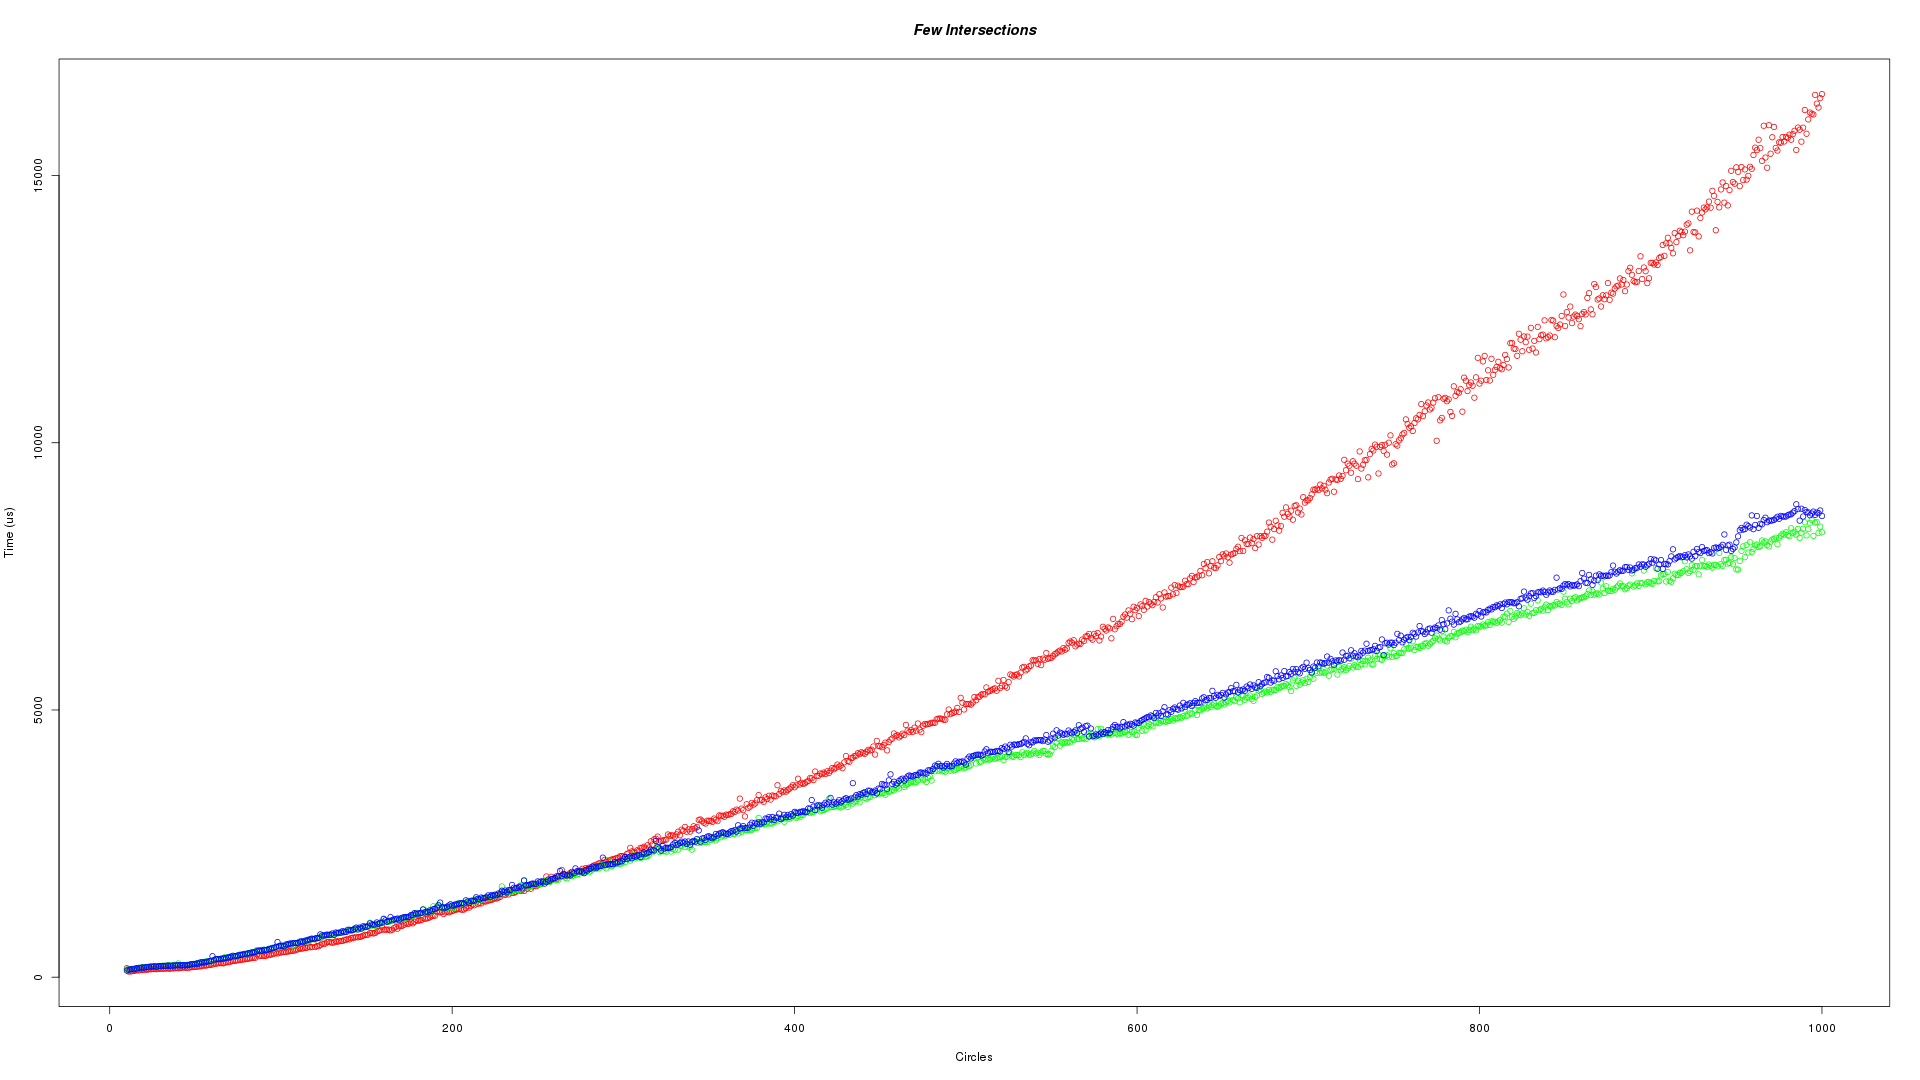
\includegraphics[width=1\textwidth]{illustraties/fewIntersections.png}
% \end{figure}
% \begin{figure}[H]
%   \centering
%   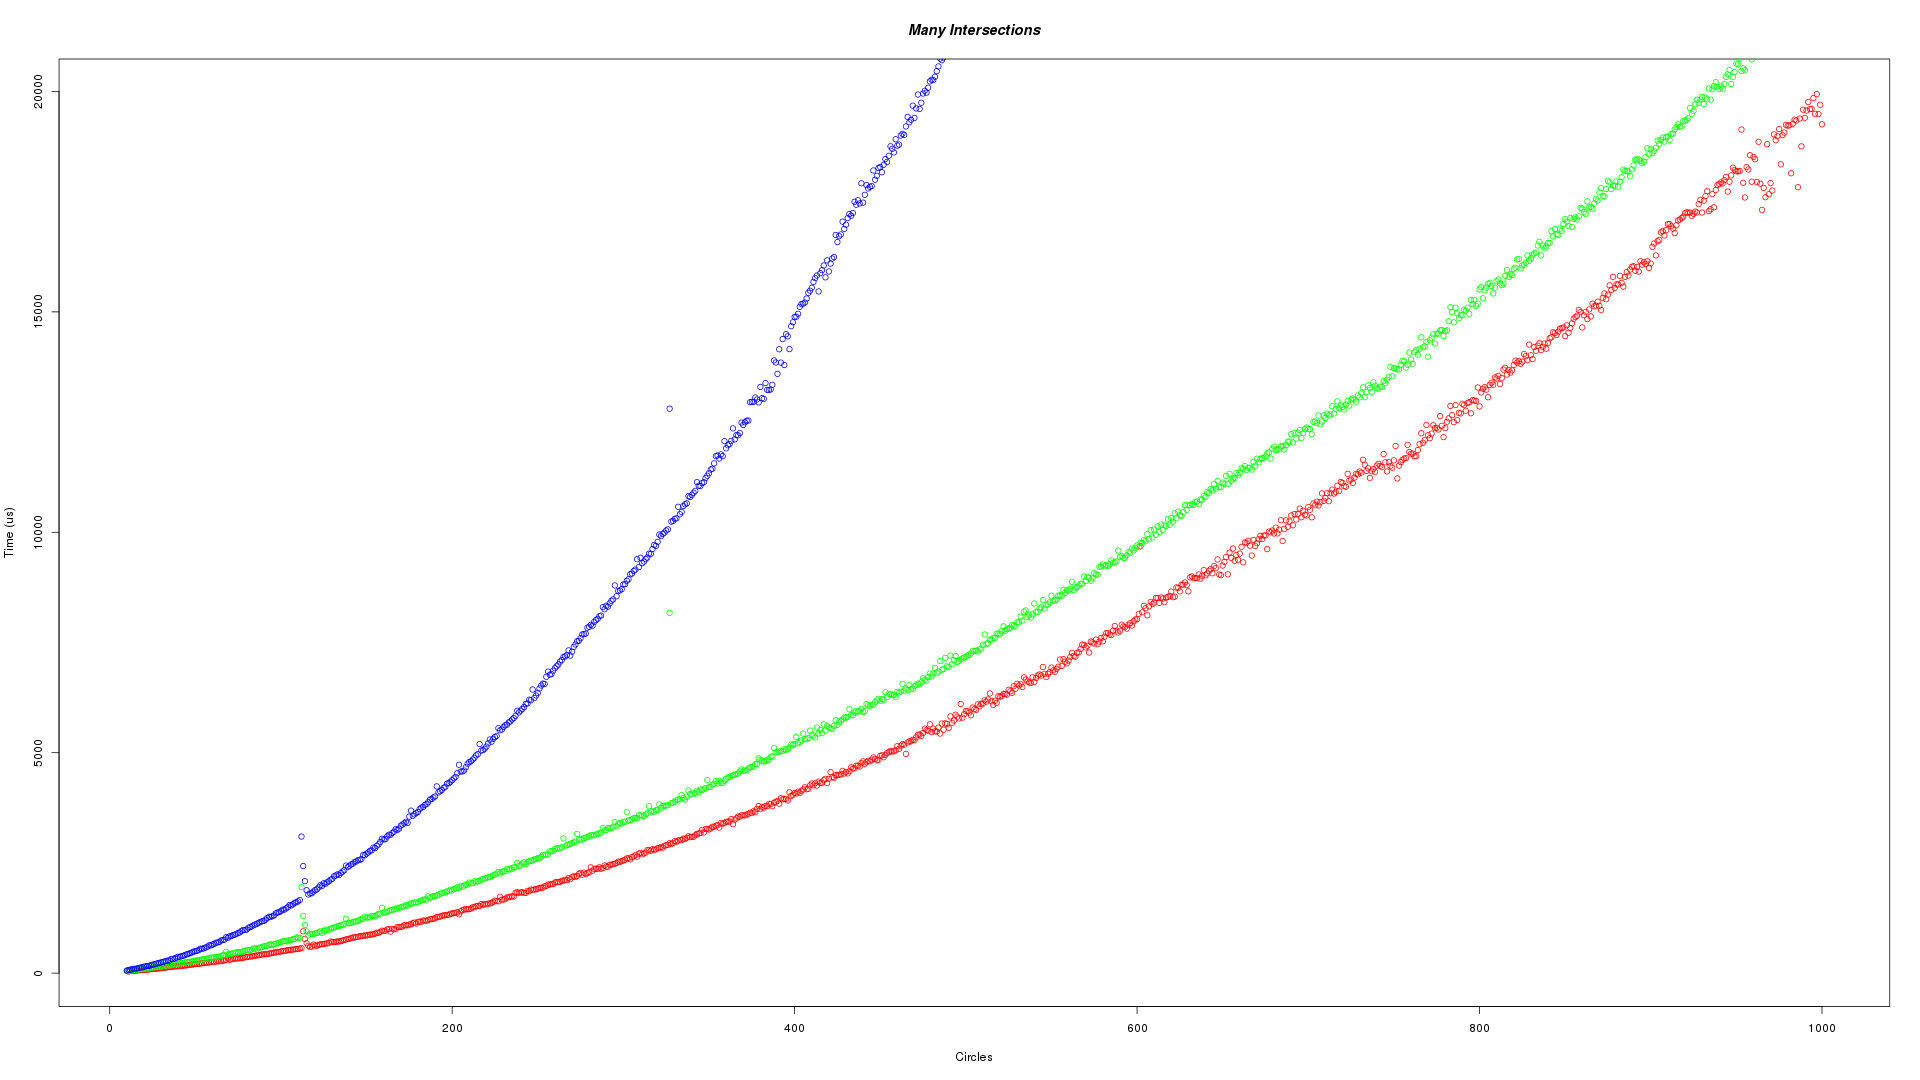
\includegraphics[width=1\textwidth]{illustraties/manyIntersections.png}
% \end{figure}
% \begin{figure}[H]
%   \centering
%   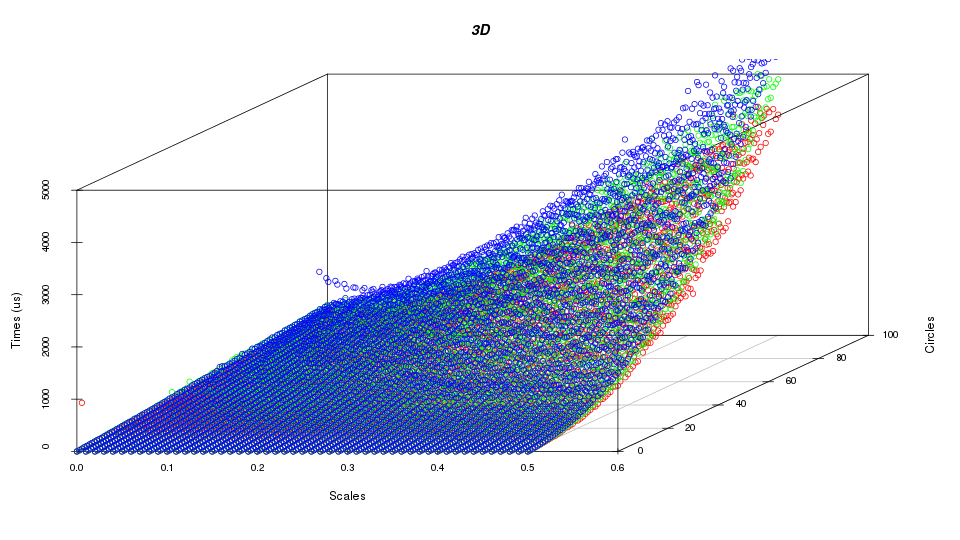
\includegraphics[width=1\textwidth]{illustraties/3DScatter.png}
% \end{figure}

% \begin{figure}[H]
%   \centering
%   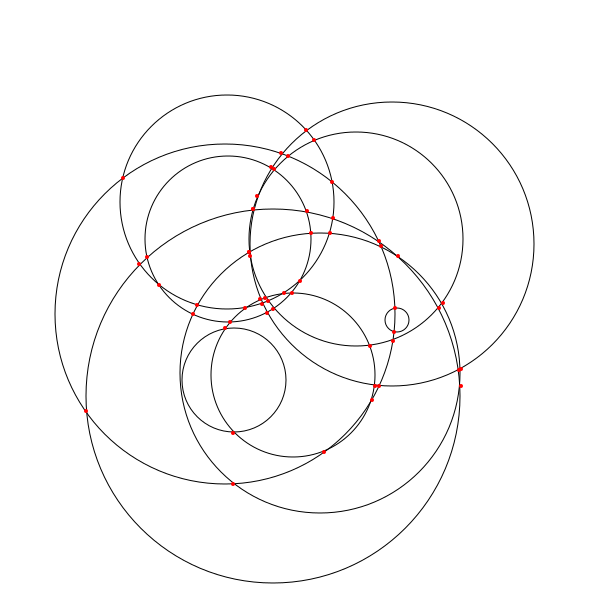
\includegraphics[width=1\textwidth]{illustraties/visuele_output.png}
% \end{figure}


\section{Resultaten}
%% \todo{grafieken}

\section{Besluit}
%% \todo{besluit}

\listoftodos

\end{document}
